We now examine the number of regions ASes peer in, how many redundant peering locations ASes maintain per peering relationship, and measure individual AS resilience to regional failure.

\subsubsection*{Geographic Peering Redundancy}
\begin{figure}[tb]
\centering
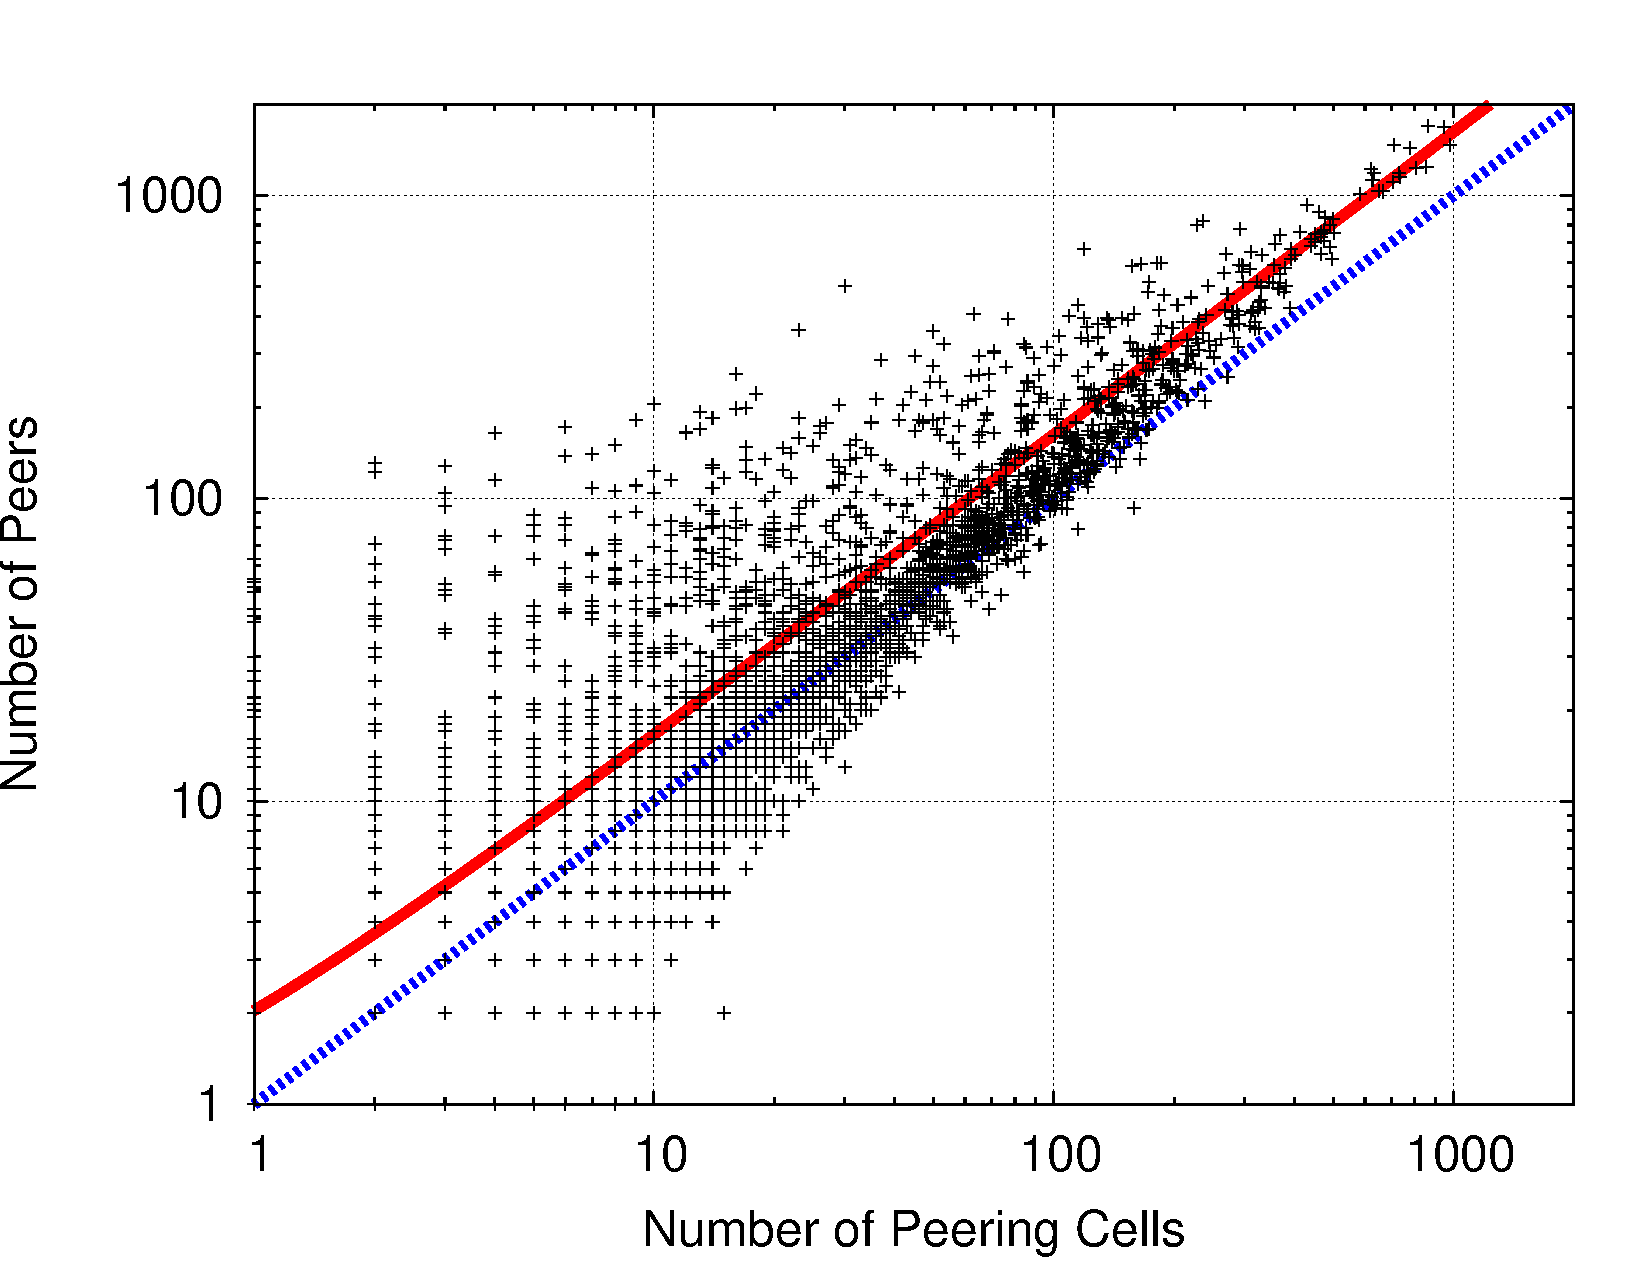
\includegraphics[width=3.25in]{scatter}
\caption[]{\label{fig:scatter} Scatter plot of observed peers to faces with peering adjacencies. Each point represents an AS which has peering in $x$ faces of the globe, with $y$ total peers. A linear regression (shown) predicts the ratio of peers:faces to be 3.1 on average.} 
\end{figure}


\begin{figure}[tb]
\centering
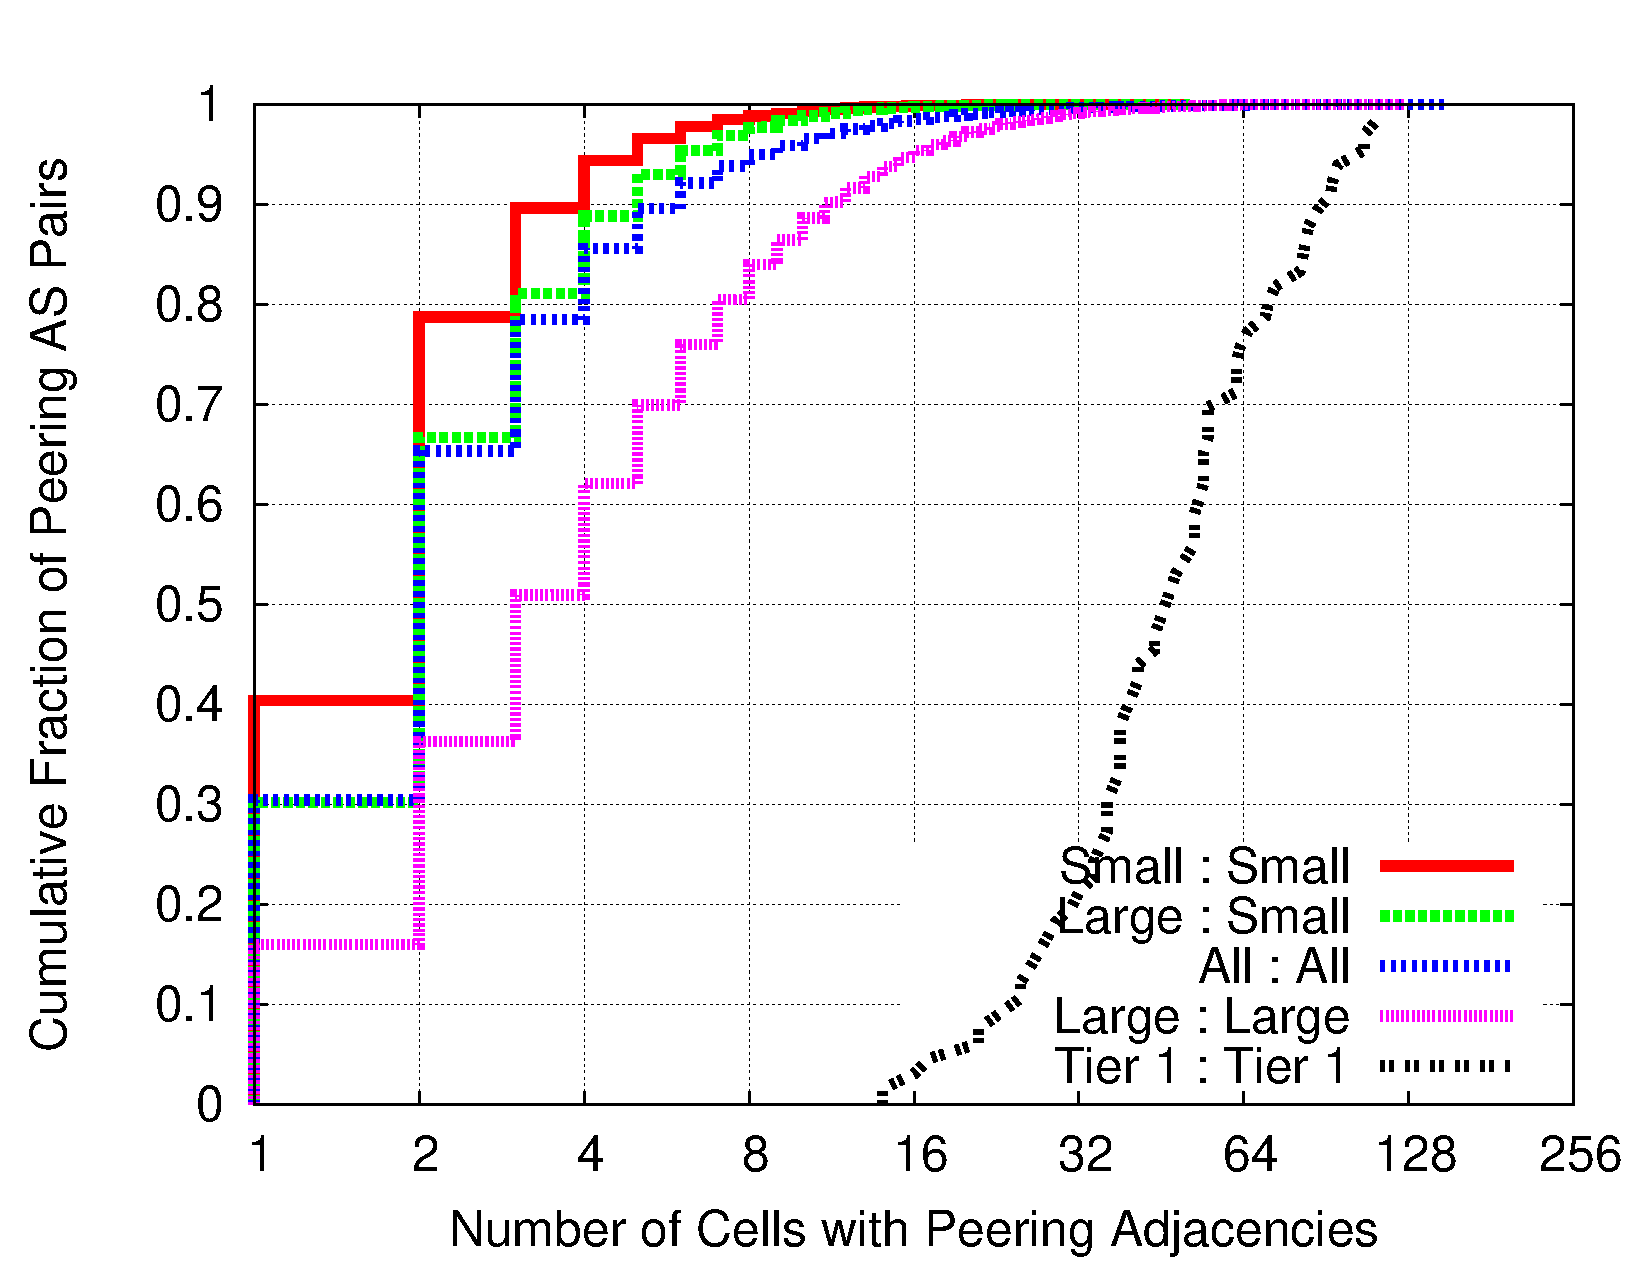
\includegraphics[width=3.25in]{peering}
\caption[]{CDF PARTY} 
\end{figure}

\subsubsection*{Quantifying Resiliance}
